\section{Installation}

\begin{frame}{System install and virtualenv}
  \begin{columns}
    \begin{column}{0.6\linewidth}
      Three advices
      \begin{enumerate}
        \item Do not install anything in the system Python
        \item Use \emph{virtual environments}
        \item Have a system for managing multiple Python versions
      \end{enumerate}

    \end{column}
    \begin{column}{0.4\linewidth}
      \begin{figure}
        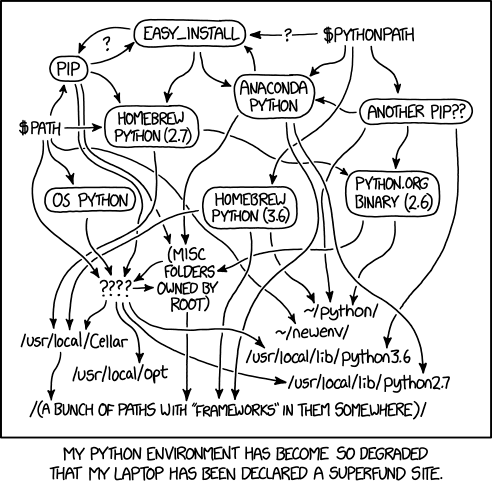
\includegraphics[width=\linewidth,keepaspectratio]{fig/python_environment}
        \caption{Randall Munroe, xkcd 1987}
      \end{figure}
    \end{column}
  \end{columns}
\end{frame}

\begin{frame}{Remember}
  \begin{itemize}
    \item You cannot see which packages that was installed directly and which was installed as dependencies
    \item Cannot, in an easy way, lock dependencies in multiple levels
  \end{itemize}
\end{frame}

\begin{frame}{Virtualenv - manage modules}
  \begin{itemize}
    \item Local package installations per enviroment/project
    \item Easy "uninstallation" by removing the folder
    \item Create in the shell or through IDE and activate with activation script
          \mintinline{shell-session}{python3 -m venv venv}\\
  \end{itemize}

  Do not forget to ignore the folder in git!
\end{frame}

\begin{frame}{pyenv - manage versions}
  \begin{itemize}
    \item Different Python versions per project
    \item Install versions independent on the system package manager
    \item Automatic activation in specific folders with \texttt{.python-version} file
    \item Install with plugins for virtualenv support
  \end{itemize}

  \vfill

  \begin{figure}
    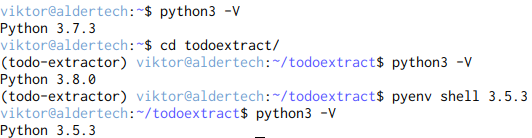
\includegraphics[width=0.8\linewidth,keepaspectratio]{fig/pyenv}
  \end{figure}
\end{frame}

\begin{frame}{pipx - manage "binaries"}
  \begin{itemize}
    \item Isolate Python program in separate venv
    \item Can both install and run directly
    \item Easy updating with \mintinline{shell-session}{pipx upgrade-all}
    \item \emph{Possible to have multiple versions of the program installed at the same time, but needs to manually symlink then}
  \end{itemize}

  Install it with \mintinline{shell-session}{pip3 install pipx}

  Is hopefully \emph{the only} package that is installed in system Python
\end{frame}
